\documentclass[11pt,openany]{article}

\usepackage{mathtools, commath}
% Packages for formatting
\usepackage[margin=1in]{geometry}
\usepackage{fancyhdr}
\usepackage{enumerate}
\usepackage{graphicx}
\usepackage{kotex}
\usepackage{amsmath}
\usepackage{amsthm}
\usepackage[dvipsnames,table]{xcolor}
\usepackage{amssymb, amsfonts}

\usepackage{arydshln} % Include this package
% Fonts
\usepackage[T1]{fontenc}
\usepackage[utf8]{inputenc}
\usepackage{newpxtext,newpxmath}
\usepackage{sectsty}

% Define colors
\definecolor{TealBlue1}{HTML}{0077c2}
\definecolor{TealBlue2}{HTML}{00a5e6}
\definecolor{TealBlue3}{HTML}{b3e0ff}
\definecolor{TealBlue4}{HTML}{00293c}
\definecolor{TealBlue5}{HTML}{e6f7ff}

\definecolor{thmcolor}{RGB}{231, 76, 60}
\definecolor{defcolor}{RGB}{52, 152, 219}
\definecolor{lemcolor}{RGB}{155, 89, 182}
\definecolor{corcolor}{RGB}{46, 204, 113}
\definecolor{procolor}{RGB}{241, 196, 15}

\usepackage{color,soul}
\usepackage{soul}
\newcommand{\mathcolorbox}[2]{\colorbox{#1}{$\displaystyle #2$}}
\usepackage{cancel}
\newcommand\crossout[3][black]{\renewcommand\CancelColor{\color{#1}}\cancelto{#2}{#3}}
\newcommand\ncrossout[2][black]{\renewcommand\CancelColor{\color{#1}}\cancel{#2}}

\usepackage{hyperref}
\usepackage{booktabs}

% Chapter formatting
\definecolor{titleTealBlue}{RGB}{0,53,128}
\usepackage{titlesec}
\titleformat{\section}
{\normalfont\sffamily\Large\bfseries\color{titleTealBlue!100!gray}}{\thesection}{1em}{}
\titleformat{\subsection}
{\normalfont\sffamily\large\bfseries\color{titleTealBlue!50!gray}}{\thesubsection}{1em}{}

%Tcolorbox
\usepackage[most]{tcolorbox}
\usepackage{multirow}
\usepackage{multicol}

\usepackage[linesnumbered,ruled]{algorithm2e}
\usepackage{algpseudocode}
\usepackage{setspace}
\SetKwComment{Comment}{/* }{ */}
\SetKwProg{Fn}{Function}{:}{end}
\SetKw{End}{end}
\SetKw{DownTo}{downto}

% Define a new environment for algorithms without line numbers
\newenvironment{algorithm2}[1][]{
	% Save the current state of the algorithm counter
	\newcounter{tempCounter}
	\setcounter{tempCounter}{\value{algocf}}
	% redefine the algorithm numbering (remove prefix)
	\renewcommand{\thealgocf}{}
	\begin{algorithm}
	}{
	\end{algorithm}
	% Restore the algorithm counter state
	\setcounter{algocf}{\value{tempCounter}}
}

\usepackage{adjustbox}
% Header and footer formatting
\pagestyle{fancy}
\fancyhead{}
\fancyhf{}
\rhead{\textcolor{TealBlue2}{\large\textbf{구체화에서 추상화에 이르는 대수학의 아름다움}}}%\rule{3cm}{0.4pt}}
\lhead{\textcolor{TealBlue2}{\large\textbf{수학의 즐거움}}}
% Define footer
\newcommand{\footer}[1]{
\begin{flushright}
	\vspace{2em}
	\includegraphics[width=2.5cm]{school_logo.jpg} \\
	\vspace{1em}
	\textcolor{TealBlue2}{\small\textbf{#1}}
\end{flushright}
}
%\rfoot{\large Department of Information Security, Cryptogrphy and Mathematics, Kookmin Uni.\includegraphics[height=1.5cm]{school_logo.jpg}}
\fancyfoot{}
\fancyfoot[C]{-\thepage-}

\newcommand{\ie}{\textnormal{i.e.}}
\newcommand{\rsa}{\mathsf{RSA}}
\newcommand{\rsacrt}{\mathsf{RSA}\textendash\mathsf{CRT}}
\newcommand{\inv}[1]{#1^{-1}}

\usepackage{amsthm}
\newtheorem{axiom}{Axiom}[section]
\newtheorem{theorem}{Theorem}
\newtheorem*{theorem*}{Theorem}
\newtheorem{proposition}[theorem]{Proposition}
\newtheorem{corollary}{Corollary}[theorem]
\newtheorem*{corollary*}{Corollary}
\newtheorem{lemma}[theorem]{Lemma}
\newtheorem*{lemma*}{Lemma}

\theoremstyle{definition}
\newtheorem{definition}{Definition}
\newtheorem*{notation*}{Notation}
\newtheorem*{definition*}{Definition}
\newtheorem*{note}{Note}
\newtheorem{remark}{Remark}
\newtheorem{example}{Example}
\newtheorem*{example*}{Example}
\newtheorem{exercise}{Exercise}[section]

%New Command
%\newcommand{\set}[1]{\left\{#1\right\}}
\newcommand{\N}{\mathbb{N}}
\newcommand{\Z}{\mathbb{Z}}
\newcommand{\Q}{\mathbb{Q}}
\newcommand{\R}{\mathbb{R}}
\newcommand{\C}{\mathbb{C}}
\newcommand{\F}{\mathbb{F}}
\newcommand{\nbhd}{\mathcal{N}}
\newcommand{\Log}{\operatorname{Log}}
\newcommand{\Arg}{\operatorname{Arg}}
\newcommand{\pv}{\operatorname{P.V.}}

\newcommand{\of}[1]{\left( #1 \right)} 
%\newcommand{\abs}[1]{\left\lvert #1 \right\rvert}
%\newcommand{\norm}[1]{\left\| #1 \right\|}

\newcommand{\sol}{\textcolor{magenta}{\bf Sol}}
\newcommand{\conjugate}[1]{\overline{#1}}

\newcommand{\res}{\operatorname{res}}
\DeclareMathOperator*{\Res}{\operatorname{Res}}

\renewcommand{\Re}{\operatorname{Re}}
\renewcommand{\Im}{\operatorname{Im}}

\newcommand{\cyclic}[1]{\langle #1 \rangle}
\newcommand{\uniform}{\overset{\$}{\leftarrow}}

\usepackage{commath}
\usepackage{caption}
%Tikzpicture
\usepackage{tikz}
\usepackage{tikz-3dplot}
\usepackage{tikz-cd}
\usetikzlibrary{
	3d, % For 3D drawing
	angles,
	arrows,
	arrows.meta,
	backgrounds,
	bending,
	calc,
	decorations.pathmorphing,
	decorations.pathreplacing,
	decorations.markings,
	fit,
	matrix,
	patterns,
	patterns.meta,
	positioning,
	quotes,
	shadows,
	shapes,
	shapes.geometric
}

\newcommand{\arrowboth}[1][]{\arrow[#1, bend left=15, myarrow]\arrow[bend left=15, myarrow, from=#1]}

\setstretch{1.25}
\begin{document}
	\pagenumbering{arabic}
	\begin{center}
		\huge\textbf{Commutative Rings}\\
		\vspace{0.5em}
		%	\Large\quad{대수학의 아름다움 서브-스터디}\\
		\vspace{0.5em}
		\normalsize{\today}\\
	\end{center}
	
\section*{The Zero Set of Simultaneous Equations Forms a Topology}
\subsection*{Definitions and Preliminaries}

- \textbf{Topological Space}: A set \( X \) with a collection \( \mathcal{T} \subseteq 2^X \) is a topological space if \( \mathcal{T} \) satisfies the following:
\begin{enumerate}
	\item \( \emptyset \in \mathcal{T} \) and \( X \in \mathcal{T} \) (inclusion of the empty set and the entire space).
	\item \( \mathcal{T} \) is closed under arbitrary unions, i.e., if \( \{ U_\alpha \}_{\alpha \in A} \subseteq \mathcal{T} \), then \( \bigcup_{\alpha \in A} U_\alpha \in \mathcal{T} \).
	\item \( \mathcal{T} \) is closed under finite intersections, i.e., if \( U_1, U_2, \ldots, U_n \in \mathcal{T} \), then \( \bigcap_{i=1}^n U_i \in \mathcal{T} \).
\end{enumerate}

\newpage
\begin{itemize}
	\item $\C[x]=\set{\sum_{i=0}^{n}a_ix^i:a_i\in\C, n\in\Z_{\geq 0}}$
	\item $\C=\set{\alpha:\alpha\in\C}$
	\item Note that $\C\subseteq\C[x]$ since $\C=\set{\alpha:\alpha\in\C}=\set{0x^n+0x^{n-1}+\cdots+\alpha x^0:\alpha\in\C}$
	\item Consider \[
	\fullfunction{\phi_\alpha}{\C[x]}{\C}{f}{f(\alpha)}
	\] and 
	\item Consider $f(x)\in\C[x]$ s.t. \[
	\fullfunction{f}{\C}{\C}{\alpha}{f(\alpha)}
	\]
	\item By the first isomorphism theorem, we have $\C[x]/\gen{x-\alpha}\simeq\C$
	\item $\gen{x-\alpha}=\set{(x-\alpha)f(x):f(x)\in\C[x]}\subseteq\C[x]$
	\item $\C[x]/\gen{x-\alpha}$;
	\begin{itemize}
		\item $p(x)=(x-\alpha)q(x)+r(x)=(x-\alpha)q(x)+r$
		\item $\C[x]/\gen{x-\alpha}=\set{r+\gen{x-\alpha}:r\in\C}$
	\end{itemize}
\end{itemize}

\adjustbox{scale=.9}{\setstretch{1.5}
\begin{tabular}{|l||c|c|} \hline
	\textbf{Mapping} & $\fullfunction{\psi_p}{\Z}{\Z_p}{n}{n\bmod p=\psi_p(n)}$ & $\fullfunction{\phi_a}{\C[x]}{\C}{f(x)}{f(a)=\phi_a(f(x))}$ \\ \hline\hline
	Additive Homo. & $\psi_p(a+b):=(a+b)\bmod p$ & $\phi_a(f+g):=f(a)+g(a)$ \\ \hline
	Multiplicative Homo. & $\psi_p(ab):=(ab)\bmod p$ & $\phi_a(fg):=f(a)g(a)$ \\ \hline
	Kernel & $\ker(\psi_p)=p\Z$ & $\ker(\phi_a)=(x-a)\C[x]$ \\ \hline
	Image & $\Z_p$ & $\C$ \\ \hline
	Ideal & $p\Z=\gen{p}$ & $(x-a)\C[x]=\gen{x-a}$ \\ \hline
	Prime Ideal & $\gen{p}$ is prime & $\gen{x-a}$ is prime \\ \hline
	Maximal Ideal & $\gen{p}$ is maximal & $\gen{x-a}$ is maximal \\ \hline
	Isomorphism & $\Z_p\simeq \Z/p\Z$ & $\C\simeq \C[x]/\gen{x-a}$ \\ \hline
	Element of Domain & $\fullfunction{n}{arg2}{arg3}{arg4}{arg5}$ & $\fullfunction{f}{\set{\gen{x-\alpha}:\alpha\in\C}}{\coprod_{\alpha}\C[x]/\gen{x-\alpha}}{\gen{x-\alpha}}{arg5}$ \\ \hline
\end{tabular}}

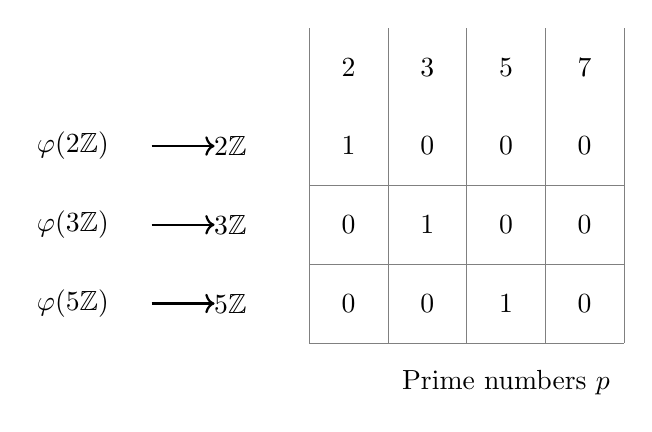
\begin{tikzpicture}[scale=1]
	
	% Draw the grid for primes
	\foreach \x in {0, 1, 2, 3, 4} {
		\draw[gray, very thin] (\x, 0) -- (\x, 4);
	}
	\foreach \y in {0, 1, 2} {
		\draw[gray, very thin] (0, \y) -- (4, \y);
	}
	
	% Labels for primes at the top
	\node at (0.5, 3.5) {2};
	\node at (1.5, 3.5) {3};
	\node at (2.5, 3.5) {5};
	\node at (3.5, 3.5) {7};
	
	% Labels for pZ on the left
	\node at (-1, 2.5) {$2\mathbb{Z}$};
	\node at (-1, 1.5) {$3\mathbb{Z}$};
	\node at (-1, 0.5) {$5\mathbb{Z}$};
	
	% Entries for pZ=2Z
	\node at (0.5, 2.5) {1}; % 1 mod 2 (for p = 2)
	\node at (1.5, 2.5) {0}; % 0 mod 3
	\node at (2.5, 2.5) {0}; % 0 mod 5
	\node at (3.5, 2.5) {0}; % 0 mod 7
	
	% Entries for pZ=3Z
	\node at (0.5, 1.5) {0}; % 0 mod 2
	\node at (1.5, 1.5) {1}; % 1 mod 3 (for p = 3)
	\node at (2.5, 1.5) {0}; % 0 mod 5
	\node at (3.5, 1.5) {0}; % 0 mod 7
	
	% Entries for pZ=5Z
	\node at (0.5, 0.5) {0}; % 0 mod 2
	\node at (1.5, 0.5) {0}; % 0 mod 3
	\node at (2.5, 0.5) {1}; % 1 mod 5 (for p = 5)
	\node at (3.5, 0.5) {0}; % 0 mod 7
	
	% Label for prime numbers
	\node at (2.5, -0.5) {Prime numbers $p$};
	
	% Arrow and description
	\draw[->, thick] (-2, 2.5) -- (-1.2, 2.5);
	\draw[->, thick] (-2, 1.5) -- (-1.2, 1.5);
	\draw[->, thick] (-2, 0.5) -- (-1.2, 0.5);
	
	\node at (-3, 2.5) {$\varphi(2\mathbb{Z})$};
	\node at (-3, 1.5) {$\varphi(3\mathbb{Z})$};
	\node at (-3, 0.5) {$\varphi(5\mathbb{Z})$};
	
\end{tikzpicture}

\end{document}
